\documentclass[11pt,a4paper]{article}
\usepackage[T1]{fontenc}
\usepackage[utf8]{inputenc}
\usepackage[margin=23mm]{geometry}
\usepackage{lmodern,microtype,xcolor,enumitem,booktabs,tabularx,longtable,needspace,array,float,tikz,listings,amsmath,amssymb}
\usetikzlibrary{arrows.meta,positioning,fit}
\usepackage[hidelinks]{hyperref}
\usepackage{xurl}
\definecolor{tueblue}{HTML}{005A9C}
\definecolor{softblue}{HTML}{EAF3F8}
\definecolor{softgray}{HTML}{F3F4F5}
\definecolor{darkgray}{HTML}{343A40}
\newcommand{\systemname}{Secure Restaurant Conveyor Delivery System}
\newcommand{\groupmembers}{Elmar Beckers, Arınç Demir, Anna Maria Petrou, Vishnu Vardhan Sirapurapu}
\newcommand{\campaign}{verification-report-20261019T150039Z}
\newcommand{\checkedinputs}{../properties}
\setlength{\parindent}{0pt}
\setlength{\parskip}{0.5em}
\setlength{\emergencystretch}{3em}
\setlist[itemize]{leftmargin=1.5em,itemsep=0.2em,topsep=0.25em}
\setlist[enumerate]{leftmargin=3.2em,itemsep=0.25em,topsep=0.25em,before=\interlinepenalty10000}
\renewcommand{\arraystretch}{1.14}
\lstdefinelanguage{mcrl}{morekeywords={sort,struct,map,var,eqn,act,proc,init,allow,block,comm,sum,lambda,if,exists,forall,nu,mu,val,true,false},sensitive=true,morecomment=[l]{\%}}
\lstdefinestyle{checked}{language=mcrl,basicstyle=\ttfamily\fontsize{8.3}{9.8}\selectfont,keywordstyle=\color{tueblue},commentstyle=\color{darkgray},numbers=left,numberstyle=\tiny\color{darkgray},numbersep=7pt,stepnumber=1,breaklines=true,breakatwhitespace=false,breakindent=1.3em,columns=fullflexible,keepspaces=true,showstringspaces=false,tabsize=4,xleftmargin=1.8em,frame=lines,framerule=0.3pt,rulecolor=\color{black!25},aboveskip=0.6em,belowskip=0.7em,captionpos=t}
\lstdefinestyle{commands}{language={},basicstyle=\ttfamily\fontsize{8.3}{9.8}\selectfont,numbers=none,breaklines=true,breakatwhitespace=false,columns=fullflexible,keepspaces=true,showstringspaces=false,frame=lines,rulecolor=\color{black!25},captionpos=t}
\pagestyle{plain}
\setcounter{tocdepth}{1}
\hypersetup{pdftitle={Secure Restaurant Conveyor Delivery System},pdfauthor={2IMF30 project group}}
\begin{document}
\begin{center}
{\Large\bfseries\color{tueblue}\systemname\par}
\vspace{0.4em}
{\large Model, requirements and native verification\par}
\vspace{0.7em}
2IMF30 System Validation, 2026--2027\par
{\small\groupmembers\par}
19 October 2026
\end{center}
{\small\textbf{AI-use disclosure.} AI assistance was used to review and revise requirements, draft and explain property formulas, prepare native verification commands and evidence records, restructure and write this report, and generate the TikZ diagram. The Boolean verification answers are computed by the mCRL2 tools.}
\tableofcontents
\clearpage

\section{System overview and purpose}
\label{sec:overview}
The system carries prepared meals from a restaurant kitchen to two tables on an indexed conveyor. A plate has an order number and a destination tag. Customers collect it from a delivery box rather than from the belt. Each box holds one plate and has an inner gate facing the conveyor, an outer gate facing the customer, and a pusher. The controller coordinates these devices so that a transfer or collection does not expose the customer to the moving belt.

An accepted order is sent to the kitchen, where a tagged plate is prepared and loaded into an empty position. The belt advances one position and stops. The kitchen and both tables receive the contents of their aligned positions. A table with a matching plate and an available box can transfer the plate, retract its pusher, close its inner gate, and open its outer gate. Otherwise it skips that visit. The kitchen and both tables report completion before movement resumes. A full box can wait for collection while its table skips later visits.

Figure~\ref{fig:physical} uses the same six positions as the checked model. The numbered nodes represent locations on the belt, rather than identities attached to plates. An advance moves each slot's contents from index $i$ to $i+1$ modulo six.

\begin{figure}[H]
\centering
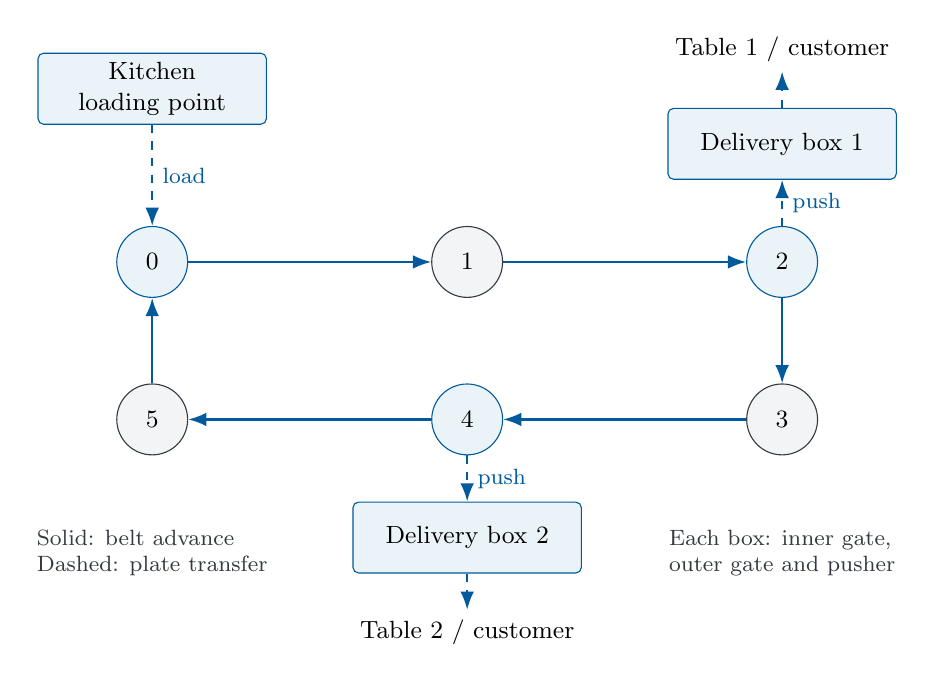
\begin{tikzpicture}[x=1cm,y=1cm,>=Latex,font=\small,
 slot/.style={circle,draw=darkgray,fill=softgray,minimum size=9mm},
 active/.style={slot,draw=tueblue,fill=softblue},
 box/.style={draw=tueblue,fill=softblue,rounded corners=2pt,align=center,minimum width=29mm,minimum height=9mm},
 flow/.style={->,thick,tueblue}, transfer/.style={->,dashed,thick,tueblue}]
\node[active] (s0) at (0,0) {0};
\node[slot] (s1) at (4,0) {1};
\node[active] (s2) at (8,0) {2};
\node[slot] (s3) at (8,-2) {3};
\node[active] (s4) at (4,-2) {4};
\node[slot] (s5) at (0,-2) {5};
\draw[flow] (s0)--(s1);
\draw[flow] (s1)--(s2);
\draw[flow] (s2)--(s3);
\draw[flow] (s3)--(s4);
\draw[flow] (s4)--(s5);
\draw[flow] (s5)--(s0);
\node[box] (kitchen) at (0,2.2) {Kitchen\\loading point};
\draw[transfer] (kitchen)--node[right,font=\footnotesize]{load}(s0);
\node[box] (b1) at (8,1.5) {Delivery box 1};
\node (t1) at (8,2.7) {Table 1 / customer};
\draw[transfer] (s2)--node[right,font=\footnotesize]{push}(b1);
\draw[transfer] (b1)--(t1);
\node[box] (b2) at (4,-3.5) {Delivery box 2};
\node (t2) at (4,-4.7) {Table 2 / customer};
\draw[transfer] (s4)--node[right,font=\footnotesize]{push}(b2);
\draw[transfer] (b2)--(t2);
\node[align=left,font=\footnotesize,text=darkgray] at (0,-3.7) {Solid: belt advance\\Dashed: plate transfer};
\node[align=left,font=\footnotesize,text=darkgray] at (8,-3.7) {Each box: inner gate,\\outer gate and pusher};
\end{tikzpicture}
\caption{The six-position verification instance: kitchen at 0, Table 1 at 2, and Table 2 at 4. Gate operations and retraction are separate steps around an atomic push.}
\label{fig:physical}
\end{figure}

Five process instances run in parallel: an order manager, a conveyor controller, a kitchen loader, and one delivery-box controller for each table. Requests and permissions synchronize so that the order manager can block unsafe operations immediately after an emergency request. Safe finishing steps, such as retraction and gate closure, can continue until all four controlled stations can receive notification. Operator clearance then authorizes a synchronized reset. The responsibilities and complete composition appear in Section~\ref{sec:code}. Parallel composition and communication follow the process-algebra approach of Groote and Mousavi~\cite[Chs.~4--5]{book}.

\section{Scope, assumptions and requirements}
\label{sec:requirements}
\subsection{Scope and bounded instance}
The product scope is one kitchen and two independently controlled, one-plate delivery boxes. Several outstanding orders and plates for the same table are allowed. A circulating belt has at most one plate per position. For verification, this is instantiated with \textbf{six belt positions, two tables, three total accepted orders, and one meal value, \texttt{Doner}}. Order numbers are 0, 1 and 2 and are not reused. The three-order limit applies over the entire execution, rather than to the number of currently outstanding orders. These are analysis bounds, not a proposed restaurant capacity policy.

Initially, the belt and boxes are empty, the belt is stopped, pushers are retracted, inner gates are open, outer gates are closed, and operation is normal. The first servicing stop must close the inner gates before movement. Although \texttt{OrderID} and \texttt{Position} are natural-number sorts, guards bound generated order numbers and the advancement counter. Station alignment is determined by fixed list indices 0, 2 and 4.

An \textbf{order} is one dish for one table and is served on one plate. A plate is \textbf{delivered} when it enters the box, and \textbf{collected} when the customer takes it through the outer gate. An \textbf{available box} is empty with its outer gate closed. A \textbf{servicing stop} begins with the synchronized round and slot snapshots while the belt is stopped. The operator's \textbf{clearance} authorizes reset; only the complete reset restores normal permissions. The model has no separate physical button-release event or second manual restart button.

Food preparation details, payments, used-plate return, temperature control, cancellation, faults in sensors or actuators, and physical timing are outside scope. Loading and delivery are atomic synchronized transitions; there is no state in which a plate is partly transferred. The model retains queued orders and plates through emergency recovery as a design choice. The suite does not separately prove complete storage preservation.

\subsection{Assumptions and meaning of progress}
The kitchen supplies correct plate tags and the equipment follows its commands. Routing is checked against the tag; matching that tag to the original accepted order is outside the verified scope. Sensor failures, mechanical timing, and partly completed transfers are not modeled.

\textbf{Can} means that a successful path exists. Such a path may include preparation, customer collection, or operator clearance. It does not promise that people will act, or that service occurs on every execution. No scheduler fairness or continued belt advancement is assumed. The progress promise in \ref{req:r7} is stronger: a normal stop must eventually advance unless a new emergency interrupts.

\subsection{Requirements}
\begin{enumerate}[label=\textbf{R\arabic*.},ref=R\arabic*,series=requirements]
  \item \label{req:r1} A box's two gates must never be open together.
  \item \label{req:r2} A plate may be delivered only to the table named on its tag.
  \item \label{req:r3} Each order may be loaded at most once and delivered at most once.
  \item \label{req:r4} The kitchen may load only into an empty loading position while the belt is stopped.
  \item \label{req:r5} A plate may enter only an empty delivery box.
  \item \label{req:r6} A pusher may start only with the correct plate aligned, the belt stopped, the inner gate open, and the outer gate closed. It must retract before the inner gate closes.
  \item \label{req:r7} The belt may start or advance only after every station has finished or skipped its work for the current stop, all inner gates are closed, and all pushers are retracted. The belt must eventually advance from each normal servicing stop, unless an emergency interrupts.
  \item \label{req:r8} Customers may collect only from an occupied box with its outer gate open and its inner gate closed.
  \item \label{req:r9} From an emergency request until reset, belt start or advance, loading, pushing, and inner-gate opening are blocked.
  \item \label{req:r10} Reset requires all controllers to have received the current emergency notification and the operator to have cleared that emergency.
  \item \label{req:r11} Every accepted order can be prepared and loaded during normal operation, without requiring an emergency.
  \item \label{req:r12} Every loaded plate can reach its tagged box without requiring an emergency. After delivery, collection must remain possible.
  \item \label{req:r13} Every emergency permits an approved reset. After reset, the belt can advance again without another emergency.
  \item \label{req:r14} Every reachable state must have a possible action. Waiting for a customer or operator is allowed if they can still act.
\end{enumerate}

\subsection*{Requirements in terms of model actions}

The following restates each requirement using the model's observable actions. A loading step combines \texttt{LoadPlate} and \texttt{PlateLoaded}; a delivery step combines \texttt{Push}, \texttt{BoxFilled}, and \texttt{PlateTransferred}. Each group happens as one synchronized step.

\begin{description}[leftmargin=3em,labelwidth=2.5em,labelsep=0.5em,itemsep=0.4em]
  \item[\ref{req:r1}] \texttt{OpenInnerGate} requires the outer gate to be closed, and \texttt{OpenOuterGate} requires the inner gate to be closed. Gate positions follow from the preceding opening and closing actions.

  \item[\ref{req:r2}] In a delivery step, the receiving table in \texttt{PlateTransferred} must match the destination carried by the plate.

  \item[\ref{req:r3}] Neither a loading step nor a delivery step may occur twice with the same order number. Emergency and reset do not erase this history.

  \item[\ref{req:r4}] Loading needs a fresh \texttt{LoadingPosition(Empty)} for the current stop and a stopped belt. The loading step consumes that empty-slot confirmation.

  \item[\ref{req:r5}] After \texttt{BoxFilled} for a table, another delivery to that box is forbidden until \texttt{BoxEmptied} occurs for the same table.

  \item[\ref{req:r6}] \texttt{ConveyorPosition} identifies the aligned plate. The \texttt{Push} step must transfer that plate with the belt stopped, the inner gate open, and the outer gate closed. Afterwards, \texttt{Retract} must precede \texttt{CloseInnerGate}.

  \item[\ref{req:r7}] The joint \texttt{RequestPermission}/\texttt{RoundPermitted} step begins a servicing stop and supplies fresh slot information. Before movement, the kitchen and both tables must each have sent \texttt{StationDone} for that stop. \texttt{StartConveyor} and \texttt{Advance} also require closed inner gates and retracted pushers. Every continuation of the stop must eventually reach \texttt{Advance} or \texttt{StartEmergency}.

  \item[\ref{req:r8}] \texttt{BoxEmptied} may occur only while the box contains an uncollected plate, its outer gate is open, and its inner gate is closed.

  \item[\ref{req:r9}] From \texttt{StartEmergency} until the synchronized reset, \texttt{StartConveyor}, \texttt{Advance}, loading, \texttt{Push}, and \texttt{OpenInnerGate} are forbidden.

  \item[\ref{req:r10}] After \texttt{StartEmergency}, all four controllers must receive the joint \texttt{EmergencyReceived} notification before \texttt{OperatorClearEmergency}. Only then may \texttt{EndEmergency} occur together with all four \texttt{EmergencyCleared} events.

  \item[\ref{req:r11}] After each \texttt{AcceptOrder}, there must be a possible continuation containing \texttt{AddPlate}, followed by a loading step for that order and table, without \texttt{StartEmergency}.

  \item[\ref{req:r12}] After each loading step, delivery of the same plate to its tagged table must be possible without \texttt{StartEmergency}. After delivery, \texttt{BoxEmptied} must remain possible until the plate is collected.

  \item[\ref{req:r13}] After \texttt{StartEmergency}, a continuation through \texttt{OperatorClearEmergency} and the synchronized reset must be possible. After every reset, a continuation to \texttt{Advance} must be possible without another \texttt{StartEmergency}.

  \item[\ref{req:r14}] After any sequence of actions, at least one further action must remain possible. Customer collection through \texttt{BoxEmptied} or clearance through \texttt{OperatorClearEmergency} also counts.
\end{description}


\subsection{Coverage choices}
The suite checks safe transport, possible service and recovery, and progress through normal stops. It does not claim complete order/plate conservation, full acceptance-to-tag identity, a full audit of skip decisions and reports, same-stop table independence, or availability of every permitted safe emergency action. The model may implement such behaviour without this report claiming it as an additional verified requirement. Historical S/F properties, the experimental R1--R22 suite, and the unregistered conditional eventual-delivery draft are outside the fourteen-property results table.

\section{Actions and Data types}
\label{sec:actions}
External interactions connect the installation with customers, kitchen staff and the operator. Physical events describe observable operations such as belt movement, gate movement and plate transfer. These observations include kitchen and staff operations; they are not limited to what a seated customer can see. Internal coordination concerns communication and control steps between the modeled components.

A label being visible in the transition system does not make it external to the installation. The model retains both physical events and selected internal coordination events so that the formulas can check the conditions for safe operation. The tables below distinguish their roles; they do not change which actions occur together.

Communication through \texttt{comm} replaces matched endpoints with a synchronized result. The \texttt{block} operator prevents unmatched endpoints from proceeding alone, while \texttt{allow} retains the specified actions and multi-actions. Hiding would remove selected action names from those labels, producing a silent step when no names remain. No hiding is used in this verification campaign. These distinctions follow the book's treatment of communication, blocking and hiding~\cite[Ch.~5]{book}; the data representations follow its data definitions~\cite[Ch.~3]{book}.

\Needspace{18\baselineskip}
\subsection{External interactions and physical events}

\begingroup
\small
\setlength{\tabcolsep}{4pt}
\renewcommand{\arraystretch}{1.13}
\begin{longtable}{@{}>{\raggedright\arraybackslash}p{0.17\textwidth}>{\raggedright\arraybackslash}p{0.32\textwidth}>{\raggedright\arraybackslash}p{0.43\textwidth}@{}}
\caption{External interactions and physical events}\label{tab:actions}\\
\toprule
\textbf{Component} & \textbf{Event} & \textbf{Meaning} \\
\midrule
\endfirsthead
\multicolumn{3}{@{}l}{\small External interactions and physical events (continued)}\\
\toprule
\textbf{Component} & \textbf{Event} & \textbf{Meaning} \\
\midrule
\endhead
\midrule
\multicolumn{3}{r@{}}{\small Continued on next page}\\
\endfoot
\bottomrule
\endlastfoot
Order manager & \texttt{AcceptOrder} & Accepts a meal and destination and stores a fresh order number internally. The event itself does not expose that number. \\
Kitchen & \texttt{AddPlate} & Prepares and associates a plate with an order number and destination. \\
Kitchen / belt & \texttt{LoadPlate}, \texttt{PlateLoaded} & One synchronized step authorizes loading and inserts the prepared plate into the empty loading slot. \\
Conveyor & \texttt{StartConveyor}, \texttt{Advance}, \texttt{StopConveyor} & Authorize movement after round completion, rotate all belt contents one indexed position, then stop. Advance carries a modulo-six movement counter. \\
Box & \texttt{OpenInnerGate}, \texttt{CloseInnerGate} & Open or close the conveyor-side gate of a specified table. \\
Box & \texttt{OpenOuterGate}, \texttt{CloseOuterGate} & Open or close the customer-side gate of a specified table. \\
Box / belt & \texttt{Push}, \texttt{BoxFilled}, \texttt{PlateTransferred} & One atomic transfer step moves the matching aligned plate from the belt into its destination box. This is the delivery event. \\
Box & \texttt{Retract} & Returns the pusher before closing the conveyor-side gate or permitting belt movement. \\
Customer / box & \texttt{BoxEmptied} & Represents customer collection from an occupied box with its customer-side gate open. \\
Order manager & \texttt{StartEmergency} & Latches the emergency request and immediately disables normal permissions, without first waiting for station notification. \\
Operator & \texttt{OperatorClearEmergency} & Records staff clearance. It does not release normal permissions. \\
Order manager & \texttt{EndEmergency} & Marks completion of emergency reset and restoration of normal permissions. It occurs together with the four controller reset events in Table~\ref{tab:coordination-actions}. \\
\end{longtable}
\endgroup

\Needspace{24\baselineskip}
\subsection{Internal coordination retained for verification}

These events describe the coordination protocol within the installation. They remain visible to the formulas, even though they are internal to the complete system. For example, a slot report exposes the information passed to a station, and a completion report records that station's reply. A synchronized step may combine roles: reset includes both \texttt{EndEmergency} and the four internal \texttt{EmergencyCleared} events.

\begingroup
\small
\setlength{\tabcolsep}{4pt}
\renewcommand{\arraystretch}{1.13}
\begin{longtable}{@{}>{\raggedright\arraybackslash}p{0.17\textwidth}>{\raggedright\arraybackslash}p{0.32\textwidth}>{\raggedright\arraybackslash}p{0.43\textwidth}@{}}
\caption{Internal coordination events retained for verification}\label{tab:coordination-actions}\\
\toprule
\textbf{Component} & \textbf{Event} & \textbf{Meaning} \\
\midrule
\endfirsthead
\multicolumn{3}{@{}l}{\small Internal coordination events (continued)}\\
\toprule
\textbf{Component} & \textbf{Event} & \textbf{Meaning} \\
\midrule
\endhead
\midrule
\multicolumn{3}{r@{}}{\small Continued on next page}\\
\endfoot
\bottomrule
\endlastfoot
Order manager / kitchen & \texttt{OrderToKitchen} & Synchronized dispatch and receipt of an accepted order and its recorded meal and destination. \\
Conveyor & \texttt{RequestPermission}, \texttt{RoundPermitted} & Begin an authorized stopped servicing round, together with the loading-slot and both table-slot reports. \\
Conveyor / kitchen & \texttt{LoadingPosition} & Reports the actual contents of the loading slot to the kitchen. \\
Conveyor / box & \texttt{ConveyorPosition} & Reports a table and the contents of the belt slot aligned with it. \\
Kitchen & \texttt{CheckPosOne} & Marks the kitchen's check of the loading-slot information it has received. \\
Station & \texttt{SendSkip} & Marks a skipped kitchen or table operation. It does not itself complete the round. Despite its name, this is a retained event rather than a blocked endpoint. \\
Station / belt & \texttt{StationDone} & Records completion of that station's work for the current round. Successful and skipped work both require this report. \\
Controllers & \texttt{EmergencyReceived} & Jointly notifies the conveyor, kitchen and both boxes once all reach their modeled notification boundaries. \\
Kitchen & \texttt{StopLoading} & Records the kitchen's transition into emergency handling after notification. \\
Controllers & \texttt{EmergencyCleared} & Jointly resets all four controllers in the same step as \texttt{EndEmergency}. \\
\end{longtable}
\endgroup

\Needspace{18\baselineskip}
\subsection{Internal communication endpoints}

The endpoints in Table~\ref{tab:internal-actions} implement synchronization between components. Unmatched send, receive, request and permit endpoints are blocked; none is named directly in R1--R14. The formulas instead match the completed events, including the internal coordination events above. Normal permissions are checked in the same step as the operation, so a permission obtained before an emergency cannot be reused afterwards.

\begingroup
\small
\setlength{\tabcolsep}{4pt}
\renewcommand{\arraystretch}{1.13}
\begin{longtable}{@{}>{\raggedright\arraybackslash}p{0.52\textwidth}>{\raggedright\arraybackslash}p{0.43\textwidth}@{}}
\caption{Internal endpoints and their synchronized results}\label{tab:internal-actions}\\
\toprule
\textbf{Endpoints} & \textbf{Result} \\
\midrule
\endfirsthead
\multicolumn{2}{@{}l}{\small Internal endpoints and their synchronized results (continued)}\\
\toprule
\textbf{Endpoints} & \textbf{Result} \\
\midrule
\endhead
\midrule
\multicolumn{2}{r@{}}{\small Continued on next page}\\
\endfoot
\bottomrule
\endlastfoot
\texttt{SendOrder} / \texttt{ReceiveOrder} & \texttt{OrderToKitchen} \\
\texttt{SendLoadingSlot} / \texttt{ReceiveLoadingSlot} & \texttt{LoadingPosition} \\
\texttt{SendTableSlot} / \texttt{ReceiveTableSlot} & \texttt{ConveyorPosition} \\
\texttt{SendPlateForLoading} / \texttt{ReceivePlateForLoading} & \texttt{PlateLoaded}, synchronized with permitted loading \\
\texttt{SendTableTransfer} / \texttt{ReceiveTableTransfer} & \texttt{PlateTransferred}, synchronized with pushing and filling the box \\
\texttt{SendStationDone} / \texttt{ReceiveStationDone} & \texttt{StationDone} \\
\texttt{RequestRound} / \texttt{PermitRound} & \texttt{RoundPermitted} \\
\texttt{RequestStartConveyor} / \texttt{PermitStartConveyor} & \texttt{StartConveyor} \\
\texttt{RequestAdvance} / \texttt{PermitAdvance} & \texttt{Advance} \\
\texttt{RequestLoadPlate} / \texttt{PermitLoadPlate} & \texttt{LoadPlate} \\
\texttt{RequestOpenInnerGate} / \texttt{PermitOpenInnerGate} & \texttt{OpenInnerGate} \\
\texttt{RequestPush} / \texttt{PermitPush} & \texttt{Push} \\
\texttt{SendEmergency} / \texttt{ReceiveEmergency} & \texttt{EmergencyReceived}, jointly for four controllers \\
\texttt{SendEmergencyReset} / \texttt{ReceiveEmergencyReset} & \texttt{EmergencyCleared}, jointly with reset \\
\end{longtable}
\endgroup

\subsection{Complete synchronized steps}
The symbol \texttt{|} joins actions in one transition. It differs from \texttt{||}, which composes processes in parallel. The formulas match the complete labels below, including their data, rather than treating one constituent as a separate transition.
\begin{itemize}
\item \textbf{Loading:} \texttt{LoadPlate(id) | PlateLoaded(plate(id,tbl))} authorizes loading and inserts the prepared plate into the belt together.
\item \textbf{Delivery:} \texttt{Push(tbl) | BoxFilled(tbl) | PlateTransferred(tbl,pl)} pushes, occupies the box, and removes the matching plate from the belt together. Retraction and gate operations follow separately.
\item \textbf{Round:} \texttt{RequestPermission | RoundPermitted} occurs with \texttt{LoadingPosition} and both \texttt{ConveyorPosition} snapshots. All stations therefore see the same stopped belt.
\item \textbf{Notification:} four \texttt{EmergencyReceived} events jointly notify the conveyor, kitchen, and both table controllers.
\item \textbf{Reset:} \texttt{EndEmergency} occurs with four \texttt{EmergencyCleared} events. Operator clearance is a separate preceding action.
\end{itemize}

\Needspace{16\baselineskip}
\subsection{Data types and storage}
Table~\ref{tab:data-types} describes the concrete representations in the checked source. In particular, a box stores occupancy rather than a plate identity; a plate's destination is carried on its belt-transfer event.
\begingroup
\small
\setlength{\tabcolsep}{4pt}
\renewcommand{\arraystretch}{1.13}
\begin{longtable}{@{}>{\raggedright\arraybackslash}p{0.17\textwidth}>{\raggedright\arraybackslash}p{0.32\textwidth}>{\raggedright\arraybackslash}p{0.43\textwidth}@{}}
\caption{Data represented in the current model}\label{tab:data-types}\\
\toprule
\textbf{Name} & \textbf{Representation} & \textbf{Meaning} \\
\midrule
\endfirsthead
\multicolumn{3}{@{}l}{\small Data represented in the current model (continued)}\\
\toprule
\textbf{Name} & \textbf{Representation} & \textbf{Meaning} \\
\midrule
\endhead
\midrule
\multicolumn{3}{r@{}}{\small Continued on next page}\\
\endfoot
\bottomrule
\endlastfoot
Meal & \texttt{Doner} & One representative meal kind in this instance. \\
TableID & \texttt{Table1}, \texttt{Table2} & Destination tables. \\
StationID & \texttt{Kitchen}, \texttt{ConveyorStation}, \texttt{TableStation(TableID)} & Stations addressed by coordination or emergency notification. \\
OrderID & Natural number & Fresh order identity; this instance accepts only 0, 1, and 2. \\
OrderEntry & Meal and TableID & Recorded meal and destination of an accepted order. \\
Plate & OrderID and TableID & Prepared plate identity and destination. The order number also identifies its single plate. \\
PlateSlot & Empty or Occupied(Plate) & Contents of one belt position or a buffered prepared plate. \\
Position & Natural number; used modulo six & Labels belt advances. Station alignment uses fixed list indices 0, 2, and 4. \\
Belt & List of six PlateSlot values & Live plate contents; initially empty. Each advance rotates all six values. \\
BoxOccupied & Boolean & Box occupancy, initially false. The box process stores occupancy rather than plate identity. \\
PosOneOccupied & Boolean & Kitchen observation of loading slot 0, despite the historical variable name. \\
GateState & Closed or Open & Both boxes initially have their conveyor-side gate open and table-side gate closed. \\
SystemMode & Normal or Emergency & Kitchen operating mode. \\
ManagerPhase & Normal, notification pending, waiting for operator, waiting for reset & Emergency latch and reset protocol of the order manager. \\
ConveyorPhase & Round ready, servicing, awaiting advance, emergency & Conveyor control state. \\
TablePhase & Waiting, opening, pushing, finishing, skipping, after reset, recovery & Delivery-box sequencing, including pusher retraction. \\
Order storage & OrderID to OrderEntry, with finite sets of pending and unassigned orders & Records accepted orders and work waiting for dispatch or loading. \\
Round replies & Finite set of StationID & Stations still required to complete the current servicing round; cancelled on emergency notification. \\
\end{longtable}
\endgroup

\Needspace{24\baselineskip}
\section{MCRL2 code}
\label{sec:code}
The complete checked source is Listing~\ref{lst:model}. Process choice (\texttt{+}) describes alternatives, action prefix (\texttt{.}) orders steps, and conditions enable the applicable alternatives. Parameter updates preserve omitted fields. Parallel composition interleaves independent actions and synchronizes the endpoint pairs listed in Table~\ref{tab:internal-actions}. These are the standard process-composition constructs described in the book~\cite[Chs.~4--5]{book}.

\begin{tabularx}{\textwidth}{@{}p{0.29\textwidth}X@{}}
\toprule
Process instance & Responsibility \\
\midrule
\texttt{OrderManager} & Stores accepted orders, dispatches pending work, grants normal permissions, latches emergencies, and coordinates notification, clearance and reset. \\
\texttt{ConveyorBelt} & Stores six live slots, publishes fresh snapshots, waits for three completion reports, and rotates the belt before stopping. \\
\texttt{KitchenLoader} & Buffers orders, prepares a plate for an empty loading slot, loads it atomically, and reports completion or a skip. \\
\texttt{DeliveryBox(Table1)} & Controls Table 1's gate interlock, aligned transfer, retraction, collection and emergency recovery. \\
\texttt{DeliveryBox(Table2)} & Runs the same controller for Table 2 with its own occupancy, gates, pusher and phase. \\
\bottomrule
\end{tabularx}

An emergency is recorded before joint notification. Permissions for movement, loading, pushing and inner-gate opening are then unavailable. A completed transfer can still retract and close its inner gate, and notification waits for safe boundaries. Recovery closes the inner gate before opening customer access. After operator clearance, reset can retain an occupied box for later collection; an empty box closes its outer gate before reopening its inner gate. This describes the source's control flow. The specific verification claims remain R1--R14.

The listing reads the versioned model directly; its bytes match the checked input, including comments and initialization. Line numbers refer to that source file; presentation wrapping does not alter it.
\lstinputlisting[style=checked,caption={Complete checked mCRL2 source (495 source lines).},label={lst:model}]{../restaurant-conveyor-delivery-system_spec.mcrl2}

\clearpage
\section{Formulas for the requirements}
\label{sec:formulas}
\subsection{Reading the formulas}
The formulas use the first-order modal $\mu$-calculus~\cite[Ch.~6]{book}. \texttt{[r] P} requires \texttt{P} after every finite path matching regular expression \texttt{r}; \texttt{<r> P} requires one such path. In path expressions, \texttt{.} concatenates, \texttt{*} allows zero or more repetitions, \texttt{!} negates an action condition, and \texttt{||} is action-condition disjunction. \texttt{true} matches any transition. Data quantifiers choose values, while \texttt{val(...)} tests a Boolean data expression. \texttt{\&\&} conjoins obligations.

For example, \texttt{[true* . A . (!B)* . C] false} forbids \texttt{C} after \texttt{A} until \texttt{B} occurs. In contrast, \texttt{[true* . A] <r . B> true} requires a possible continuation to \texttt{B} after each reachable \texttt{A}. It does not require that continuation to be selected.

A greatest fixed point, \texttt{nu}, maintains an invariant while updating a small local memory. The monitors below store an empty-slot confirmation, an aligned slot, a station-completion stage, a reset phase, or the next accepted order number. They do not store complete lifecycle histories. A least fixed point, \texttt{mu}, expresses finite progress: R7's \texttt{mu Finish} requires advancement or an emergency on every continuation from a normal stop. Its \texttt{<true> true} conjunct also rejects a deadlock before that goal.

Each following listing reads its complete versioned \texttt{.mcf} file, matching the checked revision. R12 uses the separately recorded, user-approved revision with an explicit order-ID guard described in Section~\ref{sec:verification}; the other thirteen formulas are unchanged from the initial snapshot. The \texttt{CHECK} comments name conjuncts for explanation; each file is submitted to \texttt{lts2pbes} as one formula. No conjuncts are checked as separate jobs in this campaign. The pre-run comment in R7 saying it was not yet checked records the input's state when frozen; the fresh outcome is in Section~\ref{sec:verification}.

\subsection{Observations used by the properties}
The suite checks observable system behaviour together with selected internal coordination conditions, using the distinction in Section~\ref{sec:actions}. R4 uses the round's \texttt{LoadingPosition} report to confirm an empty loading slot; R6 uses \texttt{ConveyorPosition} to identify the aligned plate. Both match the complete round label and invalidate their snapshots on advancement or the complete reset. R7 additionally observes \texttt{StationDone} to check that all three reporting stations have completed the current stop before movement.

R9 and R13 identify reset by the complete label containing \texttt{EndEmergency} and all four \texttt{EmergencyCleared} events. R10 also observes the joint \texttt{EmergencyReceived} notification to check notification, operator clearance and reset in order. These formulas therefore include protocol observations rather than using only external interactions. None names the individual blocked communication endpoints. R14 names no particular event: its \texttt{true} matches every model transition, including internal coordination, so it checks whether some action remains possible rather than whether an external action is immediately possible.

\Needspace{350pt}
\subsection{R1: Gate interlock}
\label{formula:r1}
Requirement~\ref{req:r1}: The first conjunct handles the initially open inner gate. The other two forbid opening one gate after the other has opened and before it has closed. Both directions are necessary.
\lstinputlisting[style=checked,caption={Complete formula for R1.},label={lst:r1}]{\checkedinputs/R1.mcf}

\Needspace{230pt}
\subsection{R2: Tagged destination}
\label{formula:r2}
Requirement~\ref{req:r2}: A forbidden delivery is a complete transfer whose receiving table differs from the plate tag. Correct tagging by the kitchen remains an assumption.
\lstinputlisting[style=checked,caption={Complete formula for R2.},label={lst:r2}]{\checkedinputs/R2.mcf}

\Needspace{330pt}
\subsection{R3: At-most-once processing}
\label{formula:r3}
Requirement~\ref{req:r3}: For each admitted order number, the first conjunct forbids a second load and the second forbids a second delivery. Neither history is cleared by an emergency or reset.
\lstinputlisting[style=checked,caption={Complete formula for R3.},label={lst:r3}]{\checkedinputs/R3.mcf}

\Needspace{530pt}
\subsection{R4: Safe loading}
\label{formula:r4}
Requirement~\ref{req:r4}: The Boolean monitor remembers whether the current round supplied an empty loading slot. A load consumes that confirmation; advance and reset invalidate it. The second conjunct independently forbids loading between movement and the next stop.
\lstinputlisting[style=checked,caption={Complete formula for R4.},label={lst:r4}]{\checkedinputs/R4.mcf}

\Needspace{240pt}
\subsection{R5: Empty delivery box}
\label{formula:r5}
Requirement~\ref{req:r5}: After delivery to a box, a second transfer to that box is forbidden until collection. This uses the initially empty boxes and the model's atomic filling and collection events.
\lstinputlisting[style=checked,caption={Complete formula for R5.},label={lst:r5}]{\checkedinputs/R5.mcf}

\Needspace{\textheight}
\subsection{R6: Safe pushing and retraction}
\label{formula:r6}
Requirement~\ref{req:r6}: The aligned-slot monitor records the current round's snapshot for one table. A push must consume exactly that plate and match its tag. The remaining conjuncts require a stopped belt, an open inner gate, a closed outer gate, and retraction before inner-gate closure.
\lstinputlisting[style=checked,caption={Complete formula for R6.},label={lst:r6}]{\checkedinputs/R6.mcf}

\Needspace{\textheight}
\subsection{R7: Movement barrier and stop progress}
\label{formula:r7}
Requirement~\ref{req:r7}: For each reporting station, stage 0 means no current stop, stage 1 means awaiting its completion, and stage 2 means completed. A fresh round starts stage 1; StationDone completes it. Start and advance require stage 2. Emergency, reset and advancement clear the old stop. Further conjuncts check gate closure and retraction. The final least fixed point forbids endless postponement of advancement during an uninterrupted normal stop, including deadlock. This does not audit every skip decision or duplicate report.
\lstinputlisting[style=checked,caption={Complete formula for R7.},label={lst:r7}]{\checkedinputs/R7.mcf}

\Needspace{\textheight}
\subsection{R8: Safe collection}
\label{formula:r8}
Requirement~\ref{req:r8}: The first pair of conjuncts checks initial and later occupancy. The next pair checks the initially closed and subsequently closed outer gate. The last pair checks the initially open and subsequently opened inner gate. Collection therefore requires an uncollected delivery and safe gate positions.
\lstinputlisting[style=checked,caption={Complete formula for R8.},label={lst:r8}]{\checkedinputs/R8.mcf}

\Needspace{290pt}
\subsection{R9: Emergency inhibition}
\label{formula:r9}
Requirement~\ref{req:r9}: Between the request and the complete reset, the listed unsafe transitions are forbidden. Safe finishing actions are not forbidden by this formula; it does not separately prove that every safe action remains possible.
\lstinputlisting[style=checked,caption={Complete formula for R9.},label={lst:r9}]{\checkedinputs/R9.mcf}

\Needspace{390pt}
\subsection{R10: Approved reset}
\label{formula:r10}
Requirement~\ref{req:r10}: One four-stage monitor checks normal operation, request, complete notification, and operator clearance. Only the cleared phase permits the complete reset. Other actions retain the phase. Physical repairs and a separate button protocol are outside this check.
\lstinputlisting[style=checked,caption={Complete formula for R10.},label={lst:r10}]{\checkedinputs/R10.mcf}

\Needspace{350pt}
\subsection{R11: Possible accepted-order loading}
\label{formula:r11}
Requirement~\ref{req:r11}: AcceptOrder does not expose its assigned number. The nextID counter reconstructs the model's acceptance sequence from zero. After each acceptance, a diamond requires preparation and loading of that order and table along a path without StartEmergency.
\lstinputlisting[style=checked,caption={Complete formula for R11.},label={lst:r11}]{\checkedinputs/R11.mcf}

\Needspace{360pt}
\subsection{R12: Possible delivery and continued collection access}
\label{formula:r12}
Requirement~\ref{req:r12}: After every actual load, the first conjunct requires a path to delivery of that same tagged plate without a new emergency. Collection of other plates may be used along that path. The order-ID guard makes the existing three-order bound explicit: other IDs cannot trigger a load in this model. After each delivery, the second conjunct requires collection to remain reachable from every state before collection, including states reached during emergencies.
\lstinputlisting[style=checked,caption={Complete formula for R12.},label={lst:r12}]{\checkedinputs/R12.mcf}

\Needspace{400pt}
\subsection{R13: Possible emergency recovery}
\label{formula:r13}
Requirement~\ref{req:r13}: The first conjunct requires a reset path after every request; R10 supplies its notification and clearance ordering. The second requires a path to advancement after every reset without another emergency. Both paths exclude customer collection. This is stronger than the English requirement, which does not require collection independence.
\lstinputlisting[style=checked,caption={Complete formula for R13.},label={lst:r13}]{\checkedinputs/R13.mcf}

\Needspace{190pt}
\subsection{R14: No deadlock}
\label{formula:r14}
Requirement~\ref{req:r14}: After every finite execution, some transition is enabled. Internal coordination, customer collection and operator clearance all count. This forbids terminal states. It does not require an external action to be immediately possible or guarantee eventual delivery or human participation.
\lstinputlisting[style=checked,caption={Complete formula for R14.},label={lst:r14}]{\checkedinputs/R14.mcf}

\clearpage
\section{Verification method and results}
\label{sec:verification}
\subsection{Environment and frozen revision}
This campaign starts from the current working-tree files rather than substituting results from an earlier campaign. The repository's base commit is
\begin{center}\small\texttt{42dd9c310e4e672fe21237ec6794c5372cf12917}\end{center}
The working tree was dirty: catalog, README and project configuration changes were tracked, and the current R files and supporting material were untracked. Commit identity alone therefore does not identify the checked inputs. The compact evidence under \path{verification/} records the original status, tracked diff, input hashes and native results. Large generated graphs and PBES files are omitted from Git and can be regenerated using the recorded commands. R12 has one separately frozen, user-approved revision; Table~\ref{tab:hashes} gives the selected report inputs, including that revision.

The toolset is \textbf{mCRL2 202607.0 (Release)}, installed at \path{/Applications/mCRL2.app/Contents/bin}. The host runs \textbf{macOS 27.0.1, build 26A434; Darwin 27.0.0; arm64}. Hardware is \textbf{Apple M5, Mac17,4, 10 physical and logical CPU cores, 24 GiB memory}. Tools run sequentially with their default thread settings. The recorded host command output and installed tool help are retained under \path{verification/metadata/}. Native compiled rewriting uses the installed toolchain; compilation time is included in the relevant stage.

The following working directories describe the recorded run on the verifying machine; teammates can use any fresh folder with the same relative input layout. The compact evidence is described in \path{verification/README.md}. The original campaign directory, relative to the project repository, is \path{verification-report-20261019T150039Z}. Its \path{properties/} contains the frozen formulas, its top level contains the frozen model, and commands run in its \path{run/} subdirectory. The exact absolute working directory is:
\begin{quote}\small\path{/Users/arinc/Projects/2IMF30-System-Validation/restaurant-conveyor-delivery-system/verification-report-20261019T150039Z/run}\end{quote}
The report reads the versioned model and formulas directly from the repository. Their hashes match the selected verification inputs recorded in \path{verification/inputs.sha256}. The model, all English requirements, and thirteen formulas are unchanged.

The original R12 attempt was interrupted at the user's request without a Boolean answer. Its revised first conjunct adds \texttt{val(oid < maxOrders) =>}, as R3 already does. Loading in the model requires that same bound, so IDs outside it have no triggering load and their original obligations are vacuously true. This preserves R12's meaning on this bounded model. Both versions use the same three-order model; the guard restricts the relevant formula cases, rather than reducing the model's order bound. Section~\ref{sec:r12quantification} explains the subsequent diagnostic evidence.

The revised R12 uses the same four commands from this separate working directory:
\begin{quote}\small\path{/Users/arinc/Projects/2IMF30-System-Validation/restaurant-conveyor-delivery-system/verification-report-20261019T150039Z/revisions/R12-bounded-20261019T181416Z/run}\end{quote}
Its \path{reduced.lts} links to the freshly generated graph in the original campaign. Recorded SHA-256 hashes confirm the identical model and graph. The revision runs after R13 and R14; it does not overlap another property check.

\begingroup\small
\begin{longtable}{@{}p{0.12\textwidth}p{0.82\textwidth}@{}}
\caption{SHA-256 hashes of the selected verification inputs; R12 uses its explicit order-ID guard.}\label{tab:hashes}\\
\toprule Input & SHA-256 (two consecutive halves) \\ \midrule\endfirsthead
\toprule Input & SHA-256 (continued) \\ \midrule\endhead
\bottomrule\endlastfoot
Model & \texttt{145cc14e4efcd065b7cd15068c8b0bc8}\newline\texttt{bcdaecc198070f6e4d68b8cfe5a90fae} \\
R1 & \texttt{f40f80622b4e11df184af4bbad315df7}\newline\texttt{5e334e092c3bda68afc36978f18e4dbd} \\
R2 & \texttt{347cf50e693fdac727e37ef27f0bf869}\newline\texttt{122d1dd5ce94973e8c71a7b598f0452f} \\
R3 & \texttt{30545673eb071f33b62939f53c50dc79}\newline\texttt{2c87b89ef61ed6cd77a3de9f69542bd2} \\
R4 & \texttt{3f8a1a552e009a6e95f08c7e935f8595}\newline\texttt{78e10407e7e9b7c92e4945559d82493e} \\
R5 & \texttt{ce9b88812bbd4bb8b9e8023adc4b1295}\newline\texttt{1718c188597c0f59c679e30f07b241b0} \\
R6 & \texttt{521b1682ef61d4e0e89ec8e4158e4afa}\newline\texttt{c3d2d509447bd12624f5cf9125bc83ea} \\
R7 & \texttt{200e5e76545fd892a820b99c21b7d0f2}\newline\texttt{8ae2277ce7fc5707a78feda95d6bd2a0} \\
R8 & \texttt{6f4ace6054a91bd20fc5f2f3c6deafdc}\newline\texttt{f3b868e9dccca7fadcad5faf8b2f129c} \\
R9 & \texttt{2e1e246dc9a4c4a43010ccc2a022129b}\newline\texttt{0d3c2ea51735498eef7b4316479fa5ea} \\
R10 & \texttt{eb33effa4641b6a69efe76b81beb0a1f}\newline\texttt{bec4beeed0525465913f5247bfca073a} \\
R11 & \texttt{b48861710101d87932da6a62ea10fc65}\newline\texttt{2d646395f3104a27308ab1eca4628cad} \\
R12 & \texttt{3443824ce8a989047be4f6f8c3071cc4}\newline\texttt{7aef66a535951fcf57787eb7c7d65723} \\
R13 & \texttt{fd335359dfbe70789f5b089fe045cd17}\newline\texttt{c0d9fff9c1c8290fb8d630076f697687} \\
R14 & \texttt{1bbf7f886019c586e8785356b197217e}\newline\texttt{29ddb94097f6285c420d2caccc6da207} \\
\end{longtable}
\endgroup


\subsection{Exact native commands}
The five graph commands below run once from the stated working directory. The first creates a linear process specification (LPS) using regular linearisation, followed by constant and sum elimination. The next explores the complete reachable graph, and the last minimizes it modulo strong bisimulation~\cite{mcrl22lps,lpsconstelm,lpssumelm,lps2lts,ltsconvert}. Linearisation and equivalence are developed in the book~\cite[Chs.~2, 6 and 10]{book}.
\begin{lstlisting}[style=commands,caption={Shared graph generation and reduction.},label={lst:graphcommands}]
mcrl22lps --lin-method=regular ../restaurant-conveyor-delivery-system_spec.mcrl2 model.lps
lpsconstelm model.lps model.const.lps
lpssumelm model.const.lps model.ready.lps
lps2lts --cached --rewriter=jittyc --verbose model.ready.lps complete.lts
ltsconvert --equivalence=bisim complete.lts reduced.lts
\end{lstlisting}
\Needspace{150pt}
For R1 the four property commands are exactly:
\begin{lstlisting}[style=commands,caption={Whole-formula native verification of R1.},label={lst:propertycommands}]
lts2pbes --verbose --preprocess-modal-operators --formula=../properties/R1.mcf reduced.lts R1.pbes
pbesrewr --verbose --pbes-rewriter=quantifier-one-point R1.pbes R1.one.pbes
pbesparelm --verbose R1.one.pbes R1.optimized.pbes
pbessolve --verbose --rewriter=jittyc --solve-strategy=0 R1.optimized.pbes
\end{lstlisting}
They are repeated sequentially for R2 through R14, changing only the requirement number in the formula path and output filenames. The interrupted original R12 attempt remains in that batch's records; the revised R12 repeats these same four commands separately. For a clean rerun of the selected formulas, the following Bash block gives the sequence using the graph just generated. Each \texttt{if} skips dependent stages after a tool error, then continues with the next property. A solver's \texttt{false} is a completed result and is not a tool error.
\begin{lstlisting}[style=commands,caption={Sequential checks of all fourteen whole formulas.},label={lst:batchcommands}]
for n in {1..14}; do
  if lts2pbes --verbose --preprocess-modal-operators --formula=../properties/R${n}.mcf reduced.lts R${n}.pbes &&
     pbesrewr --verbose --pbes-rewriter=quantifier-one-point R${n}.pbes R${n}.one.pbes &&
     pbesparelm --verbose R${n}.one.pbes R${n}.optimized.pbes; then
    pbessolve --verbose --rewriter=jittyc --solve-strategy=0 R${n}.optimized.pbes
  fi
done
\end{lstlisting}
The recorded \path{verification/original/verify-report-native.sh} adds standard shell sequencing, \texttt{/usr/bin/time -p}, output capture and exit-code records to these commands. It contains no custom model checker. The compact evidence contains separate \path{commands.log} and \path{stages.tsv} records for the original batch and the guarded R12 check. \path{scripts/verify-report-native.sh} runs the same native pipeline for a fresh verification. Additional \texttt{ltsinfo complete.lts} and \texttt{ltsinfo reduced.lts} commands record graph counts separately~\cite{ltsinfo}. No automatic timeout, alternate backend, historical graph, action hiding, or separate conjunct checks are used.

\subsection{Why the transformations preserve the answer}
Regular linearisation represents the parallel specification as one LPS. Constant elimination substitutes parameters proved constant from their initial values; sum elimination removes unused summation variables or substitutes equalities. These simplify representation rather than restricting reachable behaviour~\cite{mcrl22lps,lpsconstelm,lpssumelm}. The model is untimed, so no physical-time property is being preserved or checked.

\texttt{lps2lts} explores all reachable states, without a trace or state-count cutoff. \texttt{--cached} caches summand-condition evaluation within this fresh exploration; it does not load a historical state graph. \texttt{jittyc} compiles the data rewriter to speed evaluation~\cite{lps2lts}. Completion of exploration is required before any result is reported.

\texttt{ltsconvert --equivalence=bisim} merges strongly bisimilar states. Such states match each other's transitions with the same observable label and bisimilar successors. Modal $\mu$-calculus formulas cannot distinguish them, so the quotient preserves these safety, reachability, deadlock and progress checks~\cite[Chs.~2 and 6]{book}\cite{ltsconvert}. Multi-action labels and their data are retained. The formulas observe those labels and bound data rather than the file's internal state-label representation. No labels are hidden, and no weaker equivalence is used.

\texttt{lts2pbes} translates the initial-state model-checking problem into a parameterised Boolean equation system (PBES). Modal preprocessing introduces auxiliary fixed points into an equivalent formula; it changes the equation structure without changing the question~\cite{lts2pbes}. One-point rewriting substitutes equalities in quantified PBES expressions~\cite{pbesrewr}. Parameter elimination removes parameters that do not affect the solution~\cite{pbesparelm}. Finally, \texttt{pbessolve} instantiates and solves the resulting parity game. Strategy 0 disables on-the-fly solving; \texttt{jittyc} selects compiled rewriting~\cite{pbessolve}. These transformations are not assumptions about customer behaviour or scheduling.

\subsection{Measurements and outcomes}
Each stage's wall time includes input loading, computation and output writing. A property's total wall time spans all four commands and their shell overhead, excluding shared graph generation and reduction. Stage timings are measured by \texttt{/usr/bin/time -p}; total spans use the shell's timestamps. Timings are observations on this host and may differ from GUI runs or a later rerun.

A property's equation system can be larger than the reduced graph because its subformulas and monitor values create additional verification states. Reading, rewriting and saving these large files can therefore take substantial time before the solver prints its answer.
For example, the native R6 solver generated 27,387,043 Boolean equations, compared with 2,466,516 states in the shared reduced graph; its log is linked in Table~\ref{tab:results}.

A native, completed \texttt{true} is PASS and \texttt{false} is FAIL. A tool error, resource failure, missing final answer, or interruption is INCONCLUSIVE. A failed stage prevents use of its output by later stages. No earlier Boolean result or timing is imported into this campaign. Table~\ref{tab:results} links every requirement to its full formula and native evidence; shared graph work appears separately in Table~\ref{tab:graphresults}.

\begin{table}[H]
\centering
\caption{Fresh shared graph generation and reduction.}\label{tab:graphresults}
\begin{tabular}{@{}lrr@{}}
\toprule Graph & States & Transitions \\ \midrule
Complete & 5,915,640 & 17,854,674 \\
Strong-bisimulation quotient & 2,466,516 & 7,395,390 \\
\bottomrule\end{tabular}
\end{table}
\begin{table}[H]
\centering
\caption{Shared preprocessing wall times, separate from property checks.}\label{tab:preprocessing}
\begin{tabular}{@{}lrr@{}}
\toprule Stage & Seconds & Exit code \\ \midrule
\texttt{mcrl22lps} & 0.12 & 0 \\
\texttt{lpsconstelm} & 0.04 & 0 \\
\texttt{lpssumelm} & 0.01 & 0 \\
\texttt{lps2lts} & 57.02 & 0 \\
\texttt{ltsconvert} & 32.19 & 0 \\
\midrule Five-command total span & 89.439 & \\
\bottomrule\end{tabular}
\end{table}
The two additional \texttt{ltsinfo} inspections took 17.11 and 9.20 seconds and are excluded from the graph-generation and property totals. Their logs confirm the counts above.
The reported suite completed all fourteen selected native checks: 14 PASS, 0 FAIL, and 0 INCONCLUSIVE. The table contains no historical outcomes.
R12 uses the user-approved finite order-ID guard in its first conjunct. Its original attempt without an explicit ID guard was interrupted without an answer after 5596.490 seconds (93 minutes 16 seconds); the solver stage took 5261.74 seconds and exited 143. That attempt remains INCONCLUSIVE in the original records and is not counted as the revised check time. The separate revision reuses the fresh graph from this campaign, whose model and graph hashes match; it changes no English requirement or model behaviour. Both attempts are preserved in the evidence.
\Needspace{300pt}
\begingroup\small
\begin{longtable}{@{}p{0.13\textwidth}p{0.15\textwidth}p{0.21\textwidth}p{0.17\textwidth}p{0.19\textwidth}@{}}
\caption{Fresh results for complete R1--R14 formulas.}\label{tab:results}\\
\toprule Requirement & Formula & Outcome & Total check time (s) & Evidence \\ \midrule\endfirsthead
\toprule Requirement & Formula & Outcome & Total check time (s) & Evidence \\ \midrule\endhead
\bottomrule\endlastfoot
\ref{req:r1} & Listing~\ref{lst:r1} & PASS & 515.052 & \href{../verification/original/logs/R1.pbessolve.log}{R1 native log} \\
\ref{req:r2} & Listing~\ref{lst:r2} & PASS & 79.130 & \href{../verification/original/logs/R2.pbessolve.log}{R2 native log} \\
\ref{req:r3} & Listing~\ref{lst:r3} & PASS & 479.073 & \href{../verification/original/logs/R3.pbessolve.log}{R3 native log} \\
\ref{req:r4} & Listing~\ref{lst:r4} & PASS & 342.973 & \href{../verification/original/logs/R4.pbessolve.log}{R4 native log} \\
\ref{req:r5} & Listing~\ref{lst:r5} & PASS & 183.980 & \href{../verification/original/logs/R5.pbessolve.log}{R5 native log} \\
\ref{req:r6} & Listing~\ref{lst:r6} & PASS & 1426.620 & \href{../verification/original/logs/R6.pbessolve.log}{R6 native log} \\
\ref{req:r7} & Listing~\ref{lst:r7} & PASS & 1191.969 & \href{../verification/original/logs/R7.pbessolve.log}{R7 native log} \\
\ref{req:r8} & Listing~\ref{lst:r8} & PASS & 1144.686 & \href{../verification/original/logs/R8.pbessolve.log}{R8 native log} \\
\ref{req:r9} & Listing~\ref{lst:r9} & PASS & 157.185 & \href{../verification/original/logs/R9.pbessolve.log}{R9 native log} \\
\ref{req:r10} & Listing~\ref{lst:r10} & PASS & 99.893 & \href{../verification/original/logs/R10.pbessolve.log}{R10 native log} \\
\ref{req:r11} & Listing~\ref{lst:r11} & PASS & 253.523 & \href{../verification/original/logs/R11.pbessolve.log}{R11 native log} \\
\ref{req:r12} & Listing~\ref{lst:r12} & PASS & 492.164 & \href{../verification/r12-guarded/logs/R12.pbessolve.log}{R12 native log} \\
\ref{req:r13} & Listing~\ref{lst:r13} & PASS & 321.313 & \href{../verification/original/logs/R13.pbessolve.log}{R13 native log} \\
\ref{req:r14} & Listing~\ref{lst:r14} & PASS & 66.067 & \href{../verification/original/logs/R14.pbessolve.log}{R14 native log} \\
\end{longtable}
\endgroup
The evidence links point to the native solver log, or the last attempted stage after a tool failure. Commands, stage timings and exit codes are retained with the native solver logs in \path{verification/}. Large intermediate files and verbose rewriting logs are omitted from Git; the original full run remains available locally. The logs are evidence of a Boolean answer; no state-space counterexample is implied merely by a solver log.
\begingroup\small
\begin{longtable}{@{}lrrrrr@{}}
\caption{Per-property stage wall times in seconds.}\label{tab:stagetimes}\\
\toprule & \texttt{lts2pbes} & \texttt{pbesrewr} & \texttt{pbesparelm} & \texttt{pbessolve} & Total span \\ \midrule\endfirsthead
\toprule & \texttt{lts2pbes} & \texttt{pbesrewr} & \texttt{pbesparelm} & \texttt{pbessolve} & Total span \\ \midrule\endhead
\bottomrule\endlastfoot
R1 & 192.29 & 88.09 & 98.37 & 136.21 & 515.052 \\
R2 & 33.21 & 11.71 & 11.71 & 22.45 & 79.130 \\
R3 & 170.89 & 72.44 & 82.75 & 152.35 & 479.073 \\
R4 & 171.87 & 48.53 & 59.42 & 62.48 & 342.973 \\
R5 & 67.62 & 31.49 & 35.26 & 49.53 & 183.980 \\
R6 & 670.68 & 183.66 & 210.21 & 361.30 & 1426.620 \\
R7 & 634.02 & 145.81 & 173.85 & 237.15 & 1191.969 \\
R8 & 499.29 & 172.88 & 182.98 & 289.42 & 1144.686 \\
R9 & 69.79 & 24.47 & 24.23 & 38.64 & 157.185 \\
R10 & 48.08 & 13.08 & 13.89 & 24.79 & 99.893 \\
R11 & 90.39 & 37.43 & 75.18 & 46.70 & 253.523 \\
R12 & 179.31 & 80.03 & 100.32 & 131.87 & 492.164 \\
R13 & 131.86 & 55.67 & 56.48 & 77.23 & 321.313 \\
R14 & 21.18 & 11.13 & 11.93 & 21.77 & 66.067 \\
\end{longtable}
\endgroup
The stage tool times are printed to two decimal places; total spans include shell overhead and are recorded to three decimal places. A dash denotes a stage not completed or not attempted, rather than zero time.


\Needspace{350pt}
\subsection{R12: finite model and order-ID quantification}
\label{sec:r12quantification}
The model permits only three orders, but \texttt{OrderID = Nat} gives the formula a variable ranging over all natural numbers. A finite graph does not automatically make that quantifier finite. PBES instantiation considers formula-variable values as well as model states~\cite{pbessolve}. Schematically, omitting the table parameter, the original and revised equations contain:
\[
  \forall i : \mathbb{N}.\ Z(i)
  \qquad\hbox{and}\qquad
  \forall i : \mathbb{N}.\ \bigl(i \geq 3 \lor Z(i)\bigr).
\]
Here $Z(i)$ checks the delivery obligation for order $i$. For an ID such as 100, no load can occur, so the original obligation is already true. That fact is buried inside recursive equations. The solver may consider further ID values without recognizing that the remaining cases are irrelevant. The explicit guard lets the rewriter discard those cases directly, leaving only IDs 0--2 as nontrivial obligations. This is a computational distinction; the requirement and model bounds are unchanged.

To investigate, we checked both complete R12 formulas on the same isolated three-state load--deliver--collect cycle, using the same native preprocessing and solver options. The guarded formula returned \texttt{true} in 3.33 seconds, including compiled-rewriter setup, and generated 28 Boolean equations. The original formula returned no answer within a 20-second diagnostic allowance and remains INCONCLUSIVE. Idle sleep was inhibited for both runs. This toy cycle is a diagnostic fixture, not an alternative verification of the restaurant system.

We used \texttt{pbespp} to print both optimized PBESs and \texttt{diff} to compare them~\cite{pbespp}. Their only differences were the order-ID guards at the three states. This strongly implicates the quantification rather than the graph's size or laptop sleep. A finite timeout does not prove nontermination, and this test is not a full profile of the large PBES. The \href{../verification/r12-diagnostic/README.md}{diagnostic record} retains the tiny model, both formulas, native commands, printed equations, timings and logs. These diagnostic outcomes are separate from Table~\ref{tab:results}.

\clearpage
\section{Discussion and conclusion}
\label{sec:discussion}
All fourteen complete formulas returned a fresh native true answer. The results support R1--R14 for the bounded model and the stated interpretations. No requirement or formula was weakened, and no model change was made to obtain these passes.

The safety formulas constrain observable loading, transfer, gate, pusher, collection and emergency sequences within this model. Gate-state histories rely on the stated initial state. Snapshot monitors use the source's synchronized live-slot interface rather than reconstructing all six positions independently. R10 checks notification and clearance ordering; it does not establish physical repairs or button wiring.

The suite also observes selected internal coordination events, as distinguished in Section~\ref{sec:actions}. The results establish system behaviour together with those protocol conditions; they are not an exclusively external-interface verification. The communication endpoints remain composition details, while completed reports and notifications are deliberately visible. No action hiding was used to obtain the reported results.

R11--R13 express capability: each formula asks for a successful preparation, delivery or recovery continuation after each relevant trigger. A customer or operator may act along such a path. The checks do not promise that people actually participate, or that every execution delivers every meal. R14 expresses deadlock freedom but permits endless activity; only R7's normal-stop obligation explicitly excludes endless postponement before advancement or emergency. An infinite sequence of emergencies need not provide end-to-end service.

R13 retains a deliberately stronger formula than its English wording: reset and later advancement must be possible without customer collection. The additional conditional eventual-delivery draft was not part of this campaign. No result from it, the experimental suite, or legacy S/F files is included as evidence for R1--R14.

These conclusions apply to \textbf{six positions, two tables, three total accepted orders, and atomic transfers}. They do not generalize to arbitrary restaurant sizes, repeated reuse of order numbers, mechanical stopping times, sensor failures, partly transferred plates, correct kitchen tagging, or guaranteed human participation. Those need additional modeling or separate evidence. Within this boundary, retaining the checked source, formulas, hashes, commands, timings and native solver logs makes each reported outcome open to inspection. The large graphs and PBES intermediates can be regenerated rather than stored in Git.

\begin{thebibliography}{12}
\bibitem{book} J.~F.~Groote and M.~R.~Mousavi. \emph{Modeling and Analysis of Communicating Systems}. MIT Press, 2014. ISBN 9780262027717. \url{https://mitpress.mit.edu/9780262027717/modeling-and-analysis-of-communicating-systems/}.
\bibitem{mcrl22lps} mCRL2 team. \emph{mcrl22lps --- mCRL2 202607.0 user manual}. \url{https://www.mcrl2.org/web/user_manual/tools/release/mcrl22lps.html}. Accessed 19 October 2026; installed command help retained with the evidence.
\bibitem{lpsconstelm} mCRL2 team. \emph{lpsconstelm --- mCRL2 202607.0 user manual}. \url{https://www.mcrl2.org/web/user_manual/tools/release/lpsconstelm.html}. Accessed 19 October 2026; installed command help retained with the evidence.
\bibitem{lpssumelm} mCRL2 team. \emph{lpssumelm --- mCRL2 202607.0 user manual}. \url{https://www.mcrl2.org/web/user_manual/tools/release/lpssumelm.html}. Accessed 19 October 2026; installed command help retained with the evidence.
\bibitem{lps2lts} mCRL2 team. \emph{lps2lts --- mCRL2 202607.0 user manual}. \url{https://www.mcrl2.org/web/user_manual/tools/release/lps2lts.html}. Accessed 19 October 2026; installed command help retained with the evidence.
\bibitem{ltsconvert} mCRL2 team. \emph{ltsconvert --- mCRL2 202607.0 user manual}. \url{https://www.mcrl2.org/web/user_manual/tools/release/ltsconvert.html}. Accessed 19 October 2026; installed command help retained with the evidence.
\bibitem{lts2pbes} mCRL2 team. \emph{lts2pbes --- mCRL2 202607.0 user manual}. \url{https://www.mcrl2.org/web/user_manual/tools/release/lts2pbes.html}. Accessed 19 October 2026; installed command help retained with the evidence.
\bibitem{pbesrewr} mCRL2 team. \emph{pbesrewr --- mCRL2 202607.0 user manual}. \url{https://www.mcrl2.org/web/user_manual/tools/release/pbesrewr.html}. Accessed 19 October 2026; installed command help retained with the evidence.
\bibitem{pbesparelm} mCRL2 team. \emph{pbesparelm --- mCRL2 202607.0 user manual}. \url{https://www.mcrl2.org/web/user_manual/tools/release/pbesparelm.html}. Accessed 19 October 2026; installed command help retained with the evidence.
\bibitem{pbessolve} mCRL2 team. \emph{pbessolve --- mCRL2 202607.0 user manual}. \url{https://www.mcrl2.org/web/user_manual/tools/release/pbessolve.html}. Accessed 19 October 2026; installed command help retained with the evidence.
\bibitem{ltsinfo} mCRL2 team. \emph{ltsinfo --- mCRL2 202607.0 user manual}. \url{https://www.mcrl2.org/web/user_manual/tools/release/ltsinfo.html}. Accessed 19 October 2026; installed command help retained with the evidence.
\bibitem{pbespp} mCRL2 team. \emph{pbespp --- mCRL2 202607.0 command help and user manual}. \url{https://www.mcrl2.org/web/user_manual/tools/release/pbespp.html}. Installed command help consulted 19 October 2026 and retained under \path{verification/metadata/}.
\end{thebibliography}
\end{document}
